\chapter{Algoritmos de cadenas}

Este capítulo trata sobre algoritmos eficientes
para el procesamiento de cadenas.
Muchos problemas de cadenas pueden resolverse fácilmente
en tiempo $O(n^2)$, pero el desafío es
encontrar algoritmos que funcionen en tiempo $O(n)$ o $O(n \log n)$.

\index{coincidencia de patrones}

Por ejemplo, un problema fundamental de procesamiento de cadenas
es el problema de \key{coincidencia de patrones}:
dada una cadena de longitud $n$ y un patrón de longitud $m$,
nuestra tarea es encontrar las ocurrencias del patrón
en la cadena.
Por ejemplo, el patrón \texttt{ABC} ocurre dos
veces en la cadena \texttt{ABABCBABC}.

El problema de coincidencia de patrones se puede resolver fácilmente
en tiempo $O(nm)$ mediante un algoritmo de fuerza bruta que
prueba todas las posiciones donde el patrón puede
ocurrir en la cadena.
Sin embargo, en este capítulo, veremos que hay
algoritmos más eficientes que requieren solo
tiempo $O(n+m)$.

\index{cadena}

\section{Terminología de cadenas}

\index{alfabeto}

A lo largo del capítulo, asumimos que
se utiliza la indexación basada en cero en las cadenas.
Por lo tanto, una cadena \texttt{s} de longitud $n$
consiste en caracteres
$\texttt{s}[0],\texttt{s}[1],\ldots,\texttt{s}[n-1]$.
El conjunto de caracteres que pueden aparecer
en las cadenas se denomina \key{alfabeto}.
Por ejemplo, el alfabeto
$\{\texttt{A},\texttt{B},\ldots,\texttt{Z}\}$
consiste en las letras mayúsculas del inglés.

\index{subcadena}

Una \key{subcadena} es una secuencia de caracteres consecutivos
en una cadena.
Usamos la notación $\texttt{s}[a \ldots b]$
para referirnos a una subcadena de \texttt{s}
que comienza en la posición $a$ y termina en la posición $b$.
Una cadena de longitud $n$ tiene $n(n+1)/2$ subcadenas.
Por ejemplo, las subcadenas de
\texttt{ABCD} son
\texttt{A}, \texttt{B}, \texttt{C}, \texttt{D},
\texttt{AB}, \texttt{BC}, \texttt{CD},
\texttt{ABC}, \texttt{BCD} y \texttt{ABCD}.

\index{subsecuencia}

Una \key{subsecuencia} es una secuencia de
(no necesariamente consecutivos) caracteres
en una cadena en su orden original.
Una cadena de longitud $n$ tiene $2^n-1$ subsecuencias.
Por ejemplo, las subsecuencias de
\texttt{ABCD} son
\texttt{A}, \texttt{B}, \texttt{C}, \texttt{D},
\texttt{AB}, \texttt{AC}, \texttt{AD},
\texttt{BC}, \texttt{BD}, \texttt{CD},
\texttt{ABC}, \texttt{ABD}, \texttt{ACD},
\texttt{BCD} y \texttt{ABCD}.

\index{prefijo}
\index{sufijo}

Un \key{prefijo} es una subcadena que comienza al principio
de una cadena,
y un \key{sufijo} es una subcadena que termina al final
de una cadena.
Por ejemplo,
los prefijos de \texttt{ABCD} son
\texttt{A}, \texttt{AB}, \texttt{ABC} y \texttt{ABCD},
y los sufijos de \texttt{ABCD} son
\texttt{D}, \texttt{CD}, \texttt{BCD} y \texttt{ABCD}.

\index{rotación}

Una \key{rotación} se puede generar moviendo
los caracteres de una cadena uno por uno desde el principio
hasta el final (o viceversa).
Por ejemplo, las rotaciones de \texttt{ABCD} son
\texttt{ABCD}, \texttt{BCDA}, \texttt{CDAB} y \texttt{DABC}.

\index{periodo}

Un \key{periodo} es un prefijo de una cadena tal que
la cadena se puede construir repitiendo el periodo.
La última repetición puede ser parcial y contener
solo un prefijo del periodo.
Por ejemplo, el periodo más corto de
\texttt{ABCABCA} es \texttt{ABC}.

\index{borde}

Un \key{borde} es una cadena que es a la vez
un prefijo y un sufijo de una cadena.
Por ejemplo, los bordes de \texttt{ABACABA}
son \texttt{A}, \texttt{ABA} y \texttt{ABACABA}.

\index{orden lexicográfico}

Las cadenas se comparan usando el \key{orden lexicográfico}
(que corresponde al orden alfabético).
Significa que $x<y$ si $x \neq y$ y $x$ es un prefijo de $y$,
o existe una posición $k$ tal que
$x[i]=y[i]$ cuando $i<k$ y $x[k]<y[k]$.

\section{Estructura de trie}

\index{trie}

Un \key{trie} es un árbol enraizado que
mantiene un conjunto de cadenas.
Cada cadena del conjunto se almacena como
una cadena de caracteres que comienza en la raíz.
Si dos cadenas tienen un prefijo común,
también tienen una cadena común en el árbol.

Por ejemplo, considere el siguiente trie:

\begin{center}
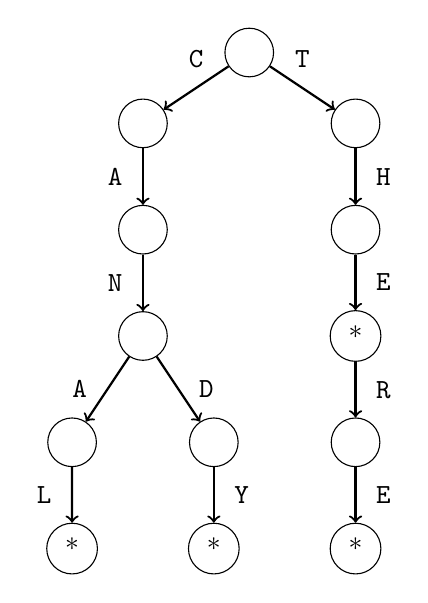
\begin{tikzpicture}[scale=0.9]
\node[draw, circle] (1) at (0,20) {$\phantom{1}$};
\node[draw, circle] (2) at (-1.5,19) {$\phantom{1}$};
\node[draw, circle] (3) at (1.5,19) {$\phantom{1}$};
\node[draw, circle] (4) at (-1.5,17.5) {$\phantom{1}$};
\node[draw, circle] (5) at (-1.5,16) {$\phantom{1}$};
\node[draw, circle] (6) at (-2.5,14.5) {$\phantom{1}$};
\node[draw, circle] (7) at (-0.5,14.5) {$\phantom{1}$};
\node[draw, circle] (8) at (-2.5,13) {*};
\node[draw, circle] (9) at (-0.5,13) {*};
\node[draw, circle] (10) at (1.5,17.5) {$\phantom{1}$};
\node[draw, circle] (11) at (1.5,16) {*};
\node[draw, circle] (12) at (1.5,14.5) {$\phantom{1}$};
\node[draw, circle] (13) at (1.5,13) {*};
\path[draw,thick,->] (1) -- node[font=\small,label=\texttt{C}] {} (2);
\path[draw,thick,->] (1) -- node[font=\small,label=\texttt{T}] {} (3);
\path[draw,thick,->] (2) -- node[font=\small,label=left:\texttt{A}] {} (4);
\path[draw,thick,->] (4) -- node[font=\small,label=left:\texttt{N}] {} (5);
\path[draw,thick,->] (5) -- node[font=\small,label=left:\texttt{A}] {} (6);
\path[draw,thick,->] (5) -- node[font=\small,label=right:\texttt{D}] {} (7);
\path[draw,thick,->] (6) -- node[font=\small,label=left:\texttt{L}] {}(8);
\path[draw,thick,->] (7) -- node[font=\small,label=right:\texttt{Y}] {} (9);
\path[draw,thick,->] (3) -- node[font=\small,label=right:\texttt{H}] {} (10);
\path[draw,thick,->] (10) -- node[font=\small,label=right:\texttt{E}] {} (11);
\path[draw,thick,->] (11) -- node[font=\small,label=right:\texttt{R}] {} (12);
\path[draw,thick,->] (12) -- node[font=\small,label=right:\texttt{E}] {} (13);
\end{tikzpicture}
\end{center}

Este trie corresponde al conjunto
$\{\texttt{CANAL},\texttt{CANDY},\texttt{THE},\texttt{THERE}\}$.
El carácter * en un nodo significa que
una cadena en el conjunto termina en el nodo.
Dicho carácter es necesario, porque una cadena
puede ser un prefijo de otra cadena.
Por ejemplo, en el trie anterior, \texttt{THE}
es un prefijo de \texttt{THERE}.

Podemos comprobar en tiempo $O(n)$ si un trie
contiene una cadena de longitud $n$,
porque podemos seguir la cadena que comienza en el nodo raíz.
También podemos agregar una cadena de longitud $n$ al trie
en tiempo $O(n)$ siguiendo primero la cadena
y luego agregando nuevos nodos al trie si es necesario.

Usando un trie, podemos encontrar
el prefijo más largo de una cadena dada
tal que el prefijo pertenezca al conjunto.
Además, al almacenar información adicional
en cada nodo,
podemos calcular el número de
cadenas que pertenecen al conjunto y tienen un
cadena dada como prefijo.

Un trie se puede almacenar en una matriz
\begin{lstlisting}
int trie[N][A];
\end{lstlisting}
donde $N$ es el número máximo de nodos
(la longitud total máxima de las cadenas en el conjunto)
y $A$ es el tamaño del alfabeto.
Los nodos de un trie están numerados
$0,1,2,\ldots$ de modo que el número de la raíz es 0,
y $\texttt{trie}[s][c]$ es el siguiente nodo en la cadena
cuando nos movemos desde el nodo $s$ usando el carácter $c$.

\section{Hashing de cadenas}

\index{hashing}
\index{hashing de cadenas}

\key{Hashing de cadenas} es una técnica que
nos permite comprobar de forma eficiente si dos
cadenas son iguales\footnote{La técnica
fue popularizada por el algoritmo de coincidencia de patrones de Karp–Rabin
\cite{kar87}.}.
La idea en el hashing de cadenas es comparar los valores hash de
cadenas en lugar de sus caracteres individuales.

\subsubsection*{Calculando valores hash}

\index{valor hash}
\index{hashing polinomial}

Un \key{valor hash} de una cadena es
un número que se calcula a partir de los caracteres
de la cadena.
Si dos cadenas son iguales,
sus valores hash también son iguales,
lo que permite comparar cadenas
basándose en sus valores hash.

Una forma habitual de implementar el hashing de cadenas
es \key{hashing polinomial}, lo que significa
que el valor hash de una cadena \texttt{s}
de longitud $n$ es
\[(\texttt{s}[0] A^{n-1} + \texttt{s}[1] A^{n-2} + \cdots + \texttt{s}[n-1] A^0) \bmod B  ,\]
donde $s[0],s[1],\ldots,s[n-1]$
se interpretan como los códigos de los caracteres de \texttt{s},
y $A$ y $B$ son constantes preseleccionadas.

Por ejemplo, los códigos de los caracteres
de \texttt{ALLEY} son:
\begin{center}
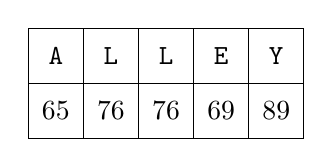
\begin{tikzpicture}[scale=0.7]
\draw (0,0) grid (5,2);

\node at (0.5, 1.5) {\texttt{A}};
\node at (1.5, 1.5) {\texttt{L}};
\node at (2.5, 1.5) {\texttt{L}};
\node at (3.5, 1.5) {\texttt{E}};
\node at (4.5, 1.5) {\texttt{Y}};

\node at (0.5, 0.5) {65};
\node at (1.5, 0.5) {76};
\node at (2.5, 0.5) {76};
\node at (3.5, 0.5) {69};
\node at (4.5, 0.5) {89};

\end{tikzpicture}
\end{center}

Por lo tanto, si $A=3$ y $B=97$, el valor hash
de \texttt{ALLEY} es
\[(65 \cdot 3^4 + 76 \cdot 3^3 + 76 \cdot 3^2 + 69 \cdot 3^1 + 89 \cdot 3^0) \bmod 97 = 52.\]

\subsubsection*{Preprocesamiento}

Usando el hashing polinomial, podemos calcular el valor hash de cualquier subcadena
de una cadena \texttt{s} en tiempo $O(1)$ después de un preprocesamiento en tiempo $O(n)$.
La idea es construir una matriz \texttt{h} tal que
$\texttt{h}[k]$ contenga el valor hash del prefijo $\texttt{s}[0 \ldots k]$.
Los valores de la matriz se pueden calcular recursivamente como sigue:
\[
\begin{array}{lcl}
\texttt{h}[0] & = & \texttt{s}[0] \\
\texttt{h}[k] & = & (\texttt{h}[k-1] A + \texttt{s}[k]) \bmod B \\
\end{array}
\]
Además, construimos una matriz \texttt{p}
donde $\texttt{p}[k]=A^k \bmod B$:
\[
\begin{array}{lcl}
\texttt{p}[0] & = & 1 \\
\texttt{p}[k] & = & (\texttt{p}[k-1] A) \bmod B. \\
\end{array}
\]
Construir estas matrices toma $O(n)$ tiempo.
Después de esto, el valor hash de cualquier subcadena
$\texttt{s}[a \ldots b]$
se puede calcular en tiempo $O(1)$ usando la fórmula
\[(\texttt{h}[b]-\texttt{h}[a-1] \texttt{p}[b-a+1]) \bmod B\]
asumiendo que $a>0$.
Si $a=0$, el valor hash es simplemente $\texttt{h}[b]$.

\subsubsection*{Usando valores hash}
Podemos comparar cadenas de manera eficiente usando valores hash.
En lugar de comparar los caracteres individuales de las cadenas,
la idea es comparar sus valores hash.
Si los valores hash son iguales,
las cadenas son \emph{probablemente} iguales,
y si los valores hash son diferentes,
las cadenas son \emph{ciertamente} diferentes.

Usando hashing, a menudo podemos hacer un algoritmo de fuerza bruta
eficiente.
Como ejemplo, considere el problema de coincidencia de patrones:
dada una cadena $s$ y un patrón $p$,
encuentre las posiciones donde $p$ ocurre en $s$.
Un algoritmo de fuerza bruta recorre todas las posiciones
donde $p$ puede ocurrir y compara las cadenas
caracter por caracter.
La complejidad temporal de tal algoritmo es $O(n^2)$.

Podemos hacer que el algoritmo de fuerza bruta sea más eficiente
usando hashing, porque el algoritmo compara
subcadenas de cadenas.
Usando hashing, cada comparación solo toma $O(1)$ tiempo,
porque solo se comparan los valores hash de las subcadenas.
Esto da como resultado un algoritmo con complejidad temporal $O(n)$,
que es la mejor complejidad temporal posible para este problema.

Combinando hashing y \emph{búsqueda binaria},
también es posible averiguar el orden lexicográfico de
dos cadenas en tiempo logarítmico.
Esto se puede hacer calculando la longitud
del prefijo común de las cadenas usando búsqueda binaria.
Una vez que conocemos la longitud del prefijo común,
solo podemos verificar el siguiente carácter después del prefijo,
porque esto determina el orden de las cadenas.

\subsubsection*{Colisiones y parámetros}

\index{colisión}

Un riesgo evidente al comparar valores hash es
una \key{colisión}, lo que significa que dos cadenas tienen
contenidos diferentes pero valores hash iguales.
En este caso, un algoritmo que se basa en
los valores hash concluye que las cadenas son iguales,
pero en realidad no lo son,
y el algoritmo puede dar resultados incorrectos.

Las colisiones siempre son posibles,
porque el número de cadenas diferentes es mayor
que el número de valores hash diferentes.
Sin embargo, la probabilidad de una colisión es pequeña
si las constantes $A$ y $B$ se eligen cuidadosamente.
Una forma habitual es elegir constantes aleatorias
cerca de $10^9$, por ejemplo de la siguiente manera:
\[
\begin{array}{lcl}
A & = & 911382323 \\
B & = & 972663749 \\
\end{array}
\]

Usando tales constantes,
el tipo \texttt{long long} se puede usar
al calcular valores hash,
porque los productos $AB$ y $BB$ cabrán en \texttt{long long}.
Pero ¿es suficiente tener alrededor de $10^9$ valores hash diferentes?

Consideremos tres escenarios donde se puede utilizar el hashing:

\textit{Escenario 1:} Las cadenas $x$ e $y$ se comparan con
entre sí.
La probabilidad de una colisión es $1/B$ asumiendo que
todos los valores hash son igualmente probables.

\textit{Escenario 2:} Una cadena $x$ se compara con cadenas
$y_1,y_2,\ldots,y_n$.
La probabilidad de una o más colisiones es

\[1-(1-\frac{1}{B})^n.\]

\textit{Escenario 3:} Todos los pares de cadenas $x_1,x_2,\ldots,x_n$
se comparan entre sí.
La probabilidad de una o más colisiones es
\[ 1 - \frac{B \cdot (B-1) \cdot (B-2) \cdots (B-n+1)}{B^n}.\]

La siguiente tabla muestra las probabilidades de colisión
cuando $n=10^6$ y el valor de $B$ varía:

\begin{center}
\begin{tabular}{rrrr}
constante $B$ & escenario 1 & escenario 2 & escenario 3 \\
\hline
$10^3$ & $0.001000$ & $1.000000$ & $1.000000$ \\
$10^6$ & $0.000001$ & $0.632121$ & $1.000000$ \\
$10^9$ & $0.000000$ & $0.001000$ & $1.000000$ \\
$10^{12}$ & $0.000000$ & $0.000000$ & $0.393469$ \\
$10^{15}$ & $0.000000$ & $0.000000$ & $0.000500$ \\
$10^{18}$ & $0.000000$ & $0.000000$ & $0.000001$ \\
\end{tabular}
\end{center}

La tabla muestra que en el escenario 1,
la probabilidad de una colisión es insignificante
cuando $B \approx 10^9$.
En el escenario 2, una colisión es posible pero la
probabilidad sigue siendo bastante pequeña.
Sin embargo, en el escenario 3 la situación es muy diferente:
una colisión ocurrirá casi siempre cuando
$B \approx 10^9$.

\index{paradoja del cumpleaños}

El fenómeno en el escenario 3 se conoce como el
\key{paradoja del cumpleaños}: si hay $n$ personas
en una habitación, la probabilidad de que \emph{algunas} dos personas
tengan el mismo cumpleaños es grande incluso si $n$ es bastante pequeño.
En hashing, en consecuencia, cuando todos los valores hash se comparan
entre sí, la probabilidad de que algunos dos
valores hash sean iguales es grande.

Podemos hacer que la probabilidad de una colisión
sea más pequeña calculando \emph{múltiples} valores hash
usando diferentes parámetros.
Es poco probable que ocurra una colisión
en todos los valores hash al mismo tiempo.
Por ejemplo, dos valores hash con parámetro
$B \approx 10^9$ corresponden a un valor hash
con parámetro $B \approx 10^{18}$,
lo que hace que la probabilidad de una colisión sea muy pequeña.

Algunas personas usan las constantes $B=2^{32}$ y $B=2^{64}$,
lo cual es conveniente, porque las operaciones con 32 y 64
enteros de bits se calculan módulo $2^{32}$ y $2^{64}$.
Sin embargo, esta \emph{no} es una buena elección, porque es posible
construir entradas que siempre generen colisiones cuando
se usan constantes de la forma $2^x$ \cite{pac13}.

\section{Algoritmo Z}

\index{Algoritmo Z}
\index{Arreglo Z}



El \key{arreglo-Z} \texttt{z} de una cadena \texttt{s}
de longitud $n$ contiene para cada $k=0,1,\ldots,n-1$
la longitud de la subcadena más larga de \texttt{s}
que comienza en la posición $k$ y es un prefijo de \texttt{s}.
Por lo tanto, $\texttt{z}[k]=p$ nos dice que
$\texttt{s}[0 \ldots p-1]$ es igual a $\texttt{s}[k \ldots k+p-1]$.
Muchos problemas de procesamiento de cadenas se pueden resolver de manera eficiente
usando el arreglo-Z.

Por ejemplo, el arreglo-Z de
\texttt{ACBACDACBACBACDA} es el siguiente:

\begin{center}
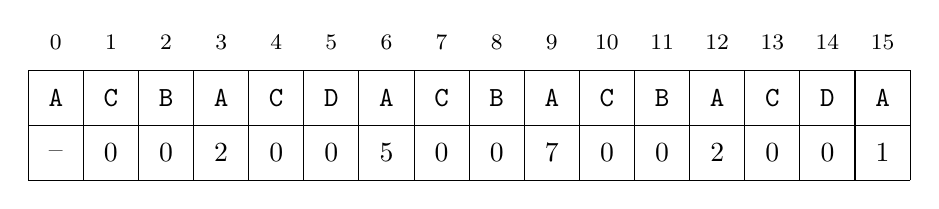
\begin{tikzpicture}[scale=0.7]
\draw (0,0) grid (16,2);

\node at (0.5, 1.5) {\texttt{A}};
\node at (1.5, 1.5) {\texttt{C}};
\node at (2.5, 1.5) {\texttt{B}};
\node at (3.5, 1.5) {\texttt{A}};
\node at (4.5, 1.5) {\texttt{C}};
\node at (5.5, 1.5) {\texttt{D}};
\node at (6.5, 1.5) {\texttt{A}};
\node at (7.5, 1.5) {\texttt{C}};
\node at (8.5, 1.5) {\texttt{B}};
\node at (9.5, 1.5) {\texttt{A}};
\node at (10.5, 1.5) {\texttt{C}};
\node at (11.5, 1.5) {\texttt{B}};
\node at (12.5, 1.5) {\texttt{A}};
\node at (13.5, 1.5) {\texttt{C}};
\node at (14.5, 1.5) {\texttt{D}};
\node at (15.5, 1.5) {\texttt{A}};

\node at (0.5, 0.5) {--};
\node at (1.5, 0.5) {0};
\node at (2.5, 0.5) {0};
\node at (3.5, 0.5) {2};
\node at (4.5, 0.5) {0};
\node at (5.5, 0.5) {0};
\node at (6.5, 0.5) {5};
\node at (7.5, 0.5) {0};
\node at (8.5, 0.5) {0};
\node at (9.5, 0.5) {7};
\node at (10.5, 0.5) {0};
\node at (11.5, 0.5) {0};
\node at (12.5, 0.5) {2};
\node at (13.5, 0.5) {0};
\node at (14.5, 0.5) {0};
\node at (15.5, 0.5) {1};

\footnotesize
\node at (0.5, 2.5) {0};
\node at (1.5, 2.5) {1};
\node at (2.5, 2.5) {2};
\node at (3.5, 2.5) {3};
\node at (4.5, 2.5) {4};
\node at (5.5, 2.5) {5};
\node at (6.5, 2.5) {6};
\node at (7.5, 2.5) {7};
\node at (8.5, 2.5) {8};
\node at (9.5, 2.5) {9};
\node at (10.5, 2.5) {10};
\node at (11.5, 2.5) {11};
\node at (12.5, 2.5) {12};
\node at (13.5, 2.5) {13};
\node at (14.5, 2.5) {14};
\node at (15.5, 2.5) {15};

\end{tikzpicture}
\end{center}

En este caso, por ejemplo, $\texttt{z}[6]=5$,
porque la subcadena \texttt{ACBAC} de longitud 5
es un prefijo de \texttt{s},
pero la subcadena \texttt{ACBACB} de longitud 6
no es un prefijo de \texttt{s}.

\subsubsection*{Descripción del algoritmo}

A continuación describimos un algoritmo,
llamado el \key{algoritmo-Z}\footnote{El algoritmo-Z
fue presentado en \cite{gus97} como el método más simple conocido
para la coincidencia de patrones en tiempo lineal, y la idea original
fue atribuida a \cite{mai84}.},
que construye de manera eficiente el arreglo-Z en tiempo $O(n)$.
El algoritmo calcula los valores del arreglo-Z
de izquierda a derecha utilizando tanto información
ya almacenada en el arreglo-Z como comparando subcadenas
caracter por caracter.

Para calcular de manera eficiente los valores del arreglo-Z,
el algoritmo mantiene un rango $[x,y]$ tal que
$\texttt{s}[x \ldots y]$ es un prefijo de \texttt{s}
e $y$ es lo más grande posible.
Dado que sabemos que $\texttt{s}[0 \ldots y-x]$
y $\texttt{s}[x \ldots y]$ son iguales,
podemos usar esta información al calcular
los valores Z para las posiciones $x+1,x+2,\ldots,y$.

En cada posición $k$, primero
verificamos el valor de $\texttt{z}[k-x]$.
Si $k+\texttt{z}[k-x]<y$, sabemos que $\texttt{z}[k]=\texttt{z}[k-x]$.
Sin embargo, si $k+\texttt{z}[k-x] \ge y$,
$\texttt{s}[0 \ldots y-k]$ es igual a
$\texttt{s}[k \ldots y]$, y para determinar el
valor de $\texttt{z}[k]$ necesitamos comparar
las subcadenas caracter por caracter.
Aún así, el algoritmo funciona en tiempo $O(n)$,
porque comenzamos a comparar en las posiciones
$y-k+1$ e $y+1$.

Por ejemplo, construyamos el siguiente arreglo-Z:

\begin{center}
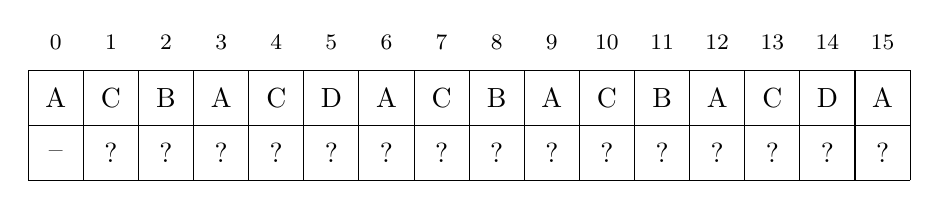
\begin{tikzpicture}[scale=0.7]
\draw (0,0) grid (16,2);

\node at (0.5, 1.5) {A};
\node at (1.5, 1.5) {C};
\node at (2.5, 1.5) {B};
\node at (3.5, 1.5) {A};
\node at (4.5, 1.5) {C};
\node at (5.5, 1.5) {D};
\node at (6.5, 1.5) {A};
\node at (7.5, 1.5) {C};
\node at (8.5, 1.5) {B};
\node at (9.5, 1.5) {A};
\node at (10.5, 1.5) {C};
\node at (11.5, 1.5) {B};
\node at (12.5, 1.5) {A};
\node at (13.5, 1.5) {C};
\node at (14.5, 1.5) {D};
\node at (15.5, 1.5) {A};

\node at (0.5, 0.5) {--};
\node at (1.5, 0.5) {?};
\node at (2.5, 0.5) {?};
\node at (3.5, 0.5) {?};
\node at (4.5, 0.5) {?};
\node at (5.5, 0.5) {?};
\node at (6.5, 0.5) {?};
\node at (7.5, 0.5) {?};
\node at (8.5, 0.5) {?};
\node at (9.5, 0.5) {?};
\node at (10.5, 0.5) {?};
\node at (11.5, 0.5) {?};
\node at (12.5, 0.5) {?};
\node at (13.5, 0.5) {?};
\node at (14.5, 0.5) {?};
\node at (15.5, 0.5) {?};

\footnotesize
\node at (0.5, 2.5) {0};
\node at (1.5, 2.5) {1};
\node at (2.5, 2.5) {2};
\node at (3.5, 2.5) {3};
\node at (4.5, 2.5) {4};
\node at (5.5, 2.5) {5};
\node at (6.5, 2.5) {6};
\node at (7.5, 2.5) {7};
\node at (8.5, 2.5) {8};
\node at (9.5, 2.5) {9};
\node at (10.5, 2.5) {10};
\node at (11.5, 2.5) {11};
\node at (12.5, 2.5) {12};
\node at (13.5, 2.5) {13};
\node at (14.5, 2.5) {14};
\node at (15.5, 2.5) {15};

\end{tikzpicture}
\end{center}

Después de calcular el valor $\texttt{z}[6]=5$,
el rango actual $[x,y]$ es $[6,10]$:
\begin{center}
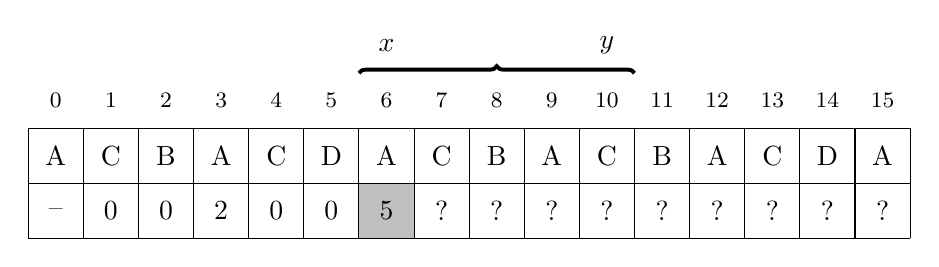
\begin{tikzpicture}[scale=0.7]
\fill[color=lightgray] (6,0) rectangle (7,1);
\draw (0,0) grid (16,2);

\node at (0.5, 1.5) {A};
\node at (1.5, 1.5) {C};
\node at (2.5, 1.5) {B};
\node at (3.5, 1.5) {A};
\node at (4.5, 1.5) {C};
\node at (5.5, 1.5) {D};
\node at (6.5, 1.5) {A};
\node at (7.5, 1.5) {C};
\node at (8.5, 1.5) {B};
\node at (9.5, 1.5) {A};
\node at (10.5, 1.5) {C};
\node at (11.5, 1.5) {B};
\node at (12.5, 1.5) {A};
\node at (13.5, 1.5) {C};
\node at (14.5, 1.5) {D};
\node at (15.5, 1.5) {A};

\node at (0.5, 0.5) {--};
\node at (1.5, 0.5) {0};
\node at (2.5, 0.5) {0};
\node at (3.5, 0.5) {2};
\node at (4.5, 0.5) {0};
\node at (5.5, 0.5) {0};
\node at (6.5, 0.5) {5};
\node at (7.5, 0.5) {?};
\node at (8.5, 0.5) {?};
\node at (9.5, 0.5) {?};
\node at (10.5, 0.5) {?};
\node at (11.5, 0.5) {?};
\node at (12.5, 0.5) {?};
\node at (13.5, 0.5) {?};
\node at (14.5, 0.5) {?};
\node at (15.5, 0.5) {?};

\draw [decoration={brace}, decorate, line width=0.5mm] (6,3.00) -- (11,3.00);

\node at (6.5,3.50) {$x$};
\node at (10.5,3.50) {$y$};


\footnotesize
\node at (0.5, 2.5) {0};
\node at (1.5, 2.5) {1};
\node at (2.5, 2.5) {2};
\node at (3.5, 2.5) {3};
\node at (4.5, 2.5) {4};
\node at (5.5, 2.5) {5};
\node at (6.5, 2.5) {6};
\node at (7.5, 2.5) {7};
\node at (8.5, 2.5) {8};
\node at (9.5, 2.5) {9};
\node at (10.5, 2.5) {10};
\node at (11.5, 2.5) {11};
\node at (12.5, 2.5) {12};
\node at (13.5, 2.5) {13};
\node at (14.5, 2.5) {14};
\node at (15.5, 2.5) {15};

\end{tikzpicture}
\end{center}

Ahora podemos calcular
los valores subsiguientes de la matriz Z
de manera eficiente,
porque sabemos que
$\texttt{s}[0 \ldots 4]$ y
$\texttt{s}[6 \ldots 10]$ son iguales.
Primero, dado que $\texttt{z}[1] = \texttt{z}[2] = 0$,
sabemos inmediatamente que también
$\texttt{z}[7] = \texttt{z}[8] = 0$:

\begin{center}
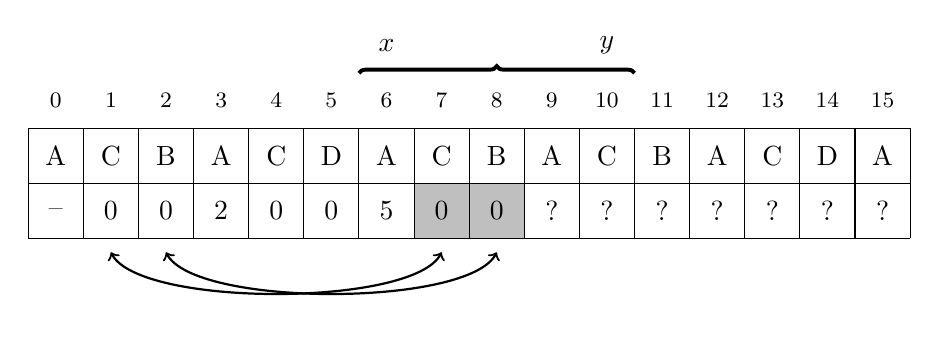
\begin{tikzpicture}[scale=0.7]
\fill[color=lightgray] (7,0) rectangle (9,1);
\draw (0,0) grid (16,2);

\node at (0.5, 1.5) {A};
\node at (1.5, 1.5) {C};
\node at (2.5, 1.5) {B};
\node at (3.5, 1.5) {A};
\node at (4.5, 1.5) {C};
\node at (5.5, 1.5) {D};
\node at (6.5, 1.5) {A};
\node at (7.5, 1.5) {C};
\node at (8.5, 1.5) {B};
\node at (9.5, 1.5) {A};
\node at (10.5, 1.5) {C};
\node at (11.5, 1.5) {B};
\node at (12.5, 1.5) {A};
\node at (13.5, 1.5) {C};
\node at (14.5, 1.5) {D};
\node at (15.5, 1.5) {A};

\node at (0.5, 0.5) {--};
\node at (1.5, 0.5) {0};
\node at (2.5, 0.5) {0};
\node at (3.5, 0.5) {2};
\node at (4.5, 0.5) {0};
\node at (5.5, 0.5) {0};
\node at (6.5, 0.5) {5};
\node at (7.5, 0.5) {0};
\node at (8.5, 0.5) {0};
\node at (9.5, 0.5) {?};
\node at (10.5, 0.5) {?};
\node at (11.5, 0.5) {?};
\node at (12.5, 0.5) {?};
\node at (13.5, 0.5) {?};
\node at (14.5, 0.5) {?};
\node at (15.5, 0.5) {?};


\draw [decoration={brace}, decorate, line width=0.5mm] (6,3.00) -- (11,3.00);

\node at (6.5,3.50) {$x$};
\node at (10.5,3.50) {$y$};


\footnotesize
\node at (0.5, 2.5) {0};
\node at (1.5, 2.5) {1};
\node at (2.5, 2.5) {2};
\node at (3.5, 2.5) {3};
\node at (4.5, 2.5) {4};
\node at (5.5, 2.5) {5};
\node at (6.5, 2.5) {6};
\node at (7.5, 2.5) {7};
\node at (8.5, 2.5) {8};
\node at (9.5, 2.5) {9};
\node at (10.5, 2.5) {10};
\node at (11.5, 2.5) {11};
\node at (12.5, 2.5) {12};
\node at (13.5, 2.5) {13};
\node at (14.5, 2.5) {14};
\node at (15.5, 2.5) {15};


\draw[thick,<->] (7.5,-0.25) .. controls (7,-1.25) and (2,-1.25) .. (1.5,-0.25);
\draw[thick,<->] (8.5,-0.25) .. controls (8,-1.25) and (3,-1.25) .. (2.5,-0.25);
\end{tikzpicture}
\end{center}

Luego, dado que $\texttt{z}[3]=2$, sabemos que $\texttt{z}[9] \ge 2$:

\begin{center}
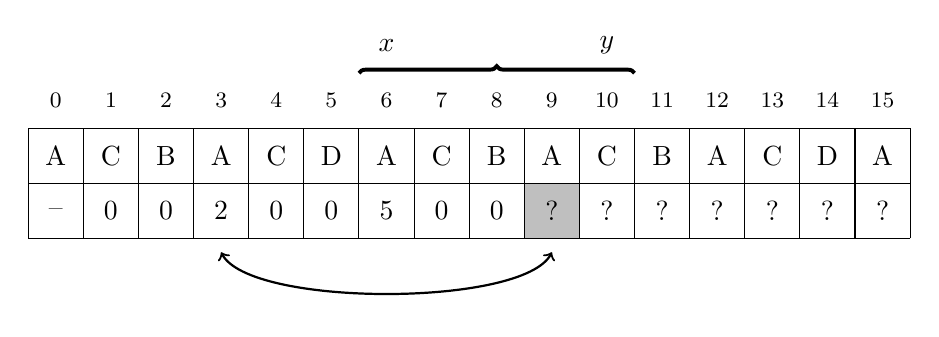
\begin{tikzpicture}[scale=0.7]
\fill[color=lightgray] (9,0) rectangle (10,1);
\draw (0,0) grid (16,2);

\node at (0.5, 1.5) {A};
\node at (1.5, 1.5) {C};
\node at (2.5, 1.5) {B};
\node at (3.5, 1.5) {A};
\node at (4.5, 1.5) {C};
\node at (5.5, 1.5) {D};
\node at (6.5, 1.5) {A};
\node at (7.5, 1.5) {C};
\node at (8.5, 1.5) {B};
\node at (9.5, 1.5) {A};
\node at (10.5, 1.5) {C};
\node at (11.5, 1.5) {B};
\node at (12.5, 1.5) {A};
\node at (13.5, 1.5) {C};
\node at (14.5, 1.5) {D};
\node at (15.5, 1.5) {A};

\node at (0.5, 0.5) {--};
\node at (1.5, 0.5) {0};
\node at (2.5, 0.5) {0};
\node at (3.5, 0.5) {2};
\node at (4.5, 0.5) {0};
\node at (5.5, 0.5) {0};
\node at (6.5, 0.5) {5};
\node at (7.5, 0.5) {0};
\node at (8.5, 0.5) {0};
\node at (9.5, 0.5) {?};
\node at (10.5, 0.5) {?};
\node at (11.5, 0.5) {?};
\node at (12.5, 0.5) {?};
\node at (13.5, 0.5) {?};
\node at (14.5, 0.5) {?};
\node at (15.5, 0.5) {?};

\draw [decoration={brace}, decorate, line width=0.5mm] (6,3.00) -- (11,3.00);

\node at (6.5,3.50) {$x$};
\node at (10.5,3.50) {$y$};
\footnotesize
\node at (0.5, 2.5) {0};
\node at (1.5, 2.5) {1};
\node at (2.5, 2.5) {2};
\node at (3.5, 2.5) {3};
\node at (4.5, 2.5) {4};
\node at (5.5, 2.5) {5};
\node at (6.5, 2.5) {6};
\node at (7.5, 2.5) {7};
\node at (8.5, 2.5) {8};
\node at (9.5, 2.5) {9};
\node at (10.5, 2.5) {10};
\node at (11.5, 2.5) {11};
\node at (12.5, 2.5) {12};
\node at (13.5, 2.5) {13};
\node at (14.5, 2.5) {14};
\node at (15.5, 2.5) {15};

\draw[thick,<->] (9.5,-0.25) .. controls (9,-1.25) and (4,-1.25) .. (3.5,-0.25);
\end{tikzpicture}
\end{center}

Sin embargo, no tenemos información sobre la cadena
después de la posición 10, por lo que necesitamos comparar las subcadenas
caracter por caracter:

\begin{center}
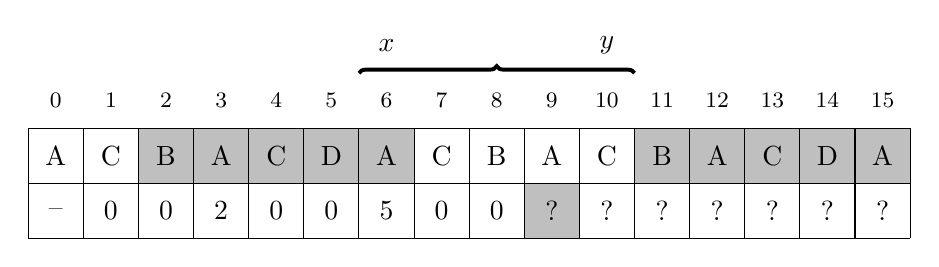
\begin{tikzpicture}[scale=0.7]
\fill[color=lightgray] (9,0) rectangle (10,1);
\fill[color=lightgray] (2,1) rectangle (7,2);
\fill[color=lightgray] (11,1) rectangle (16,2);


\draw (0,0) grid (16,2);

\node at (0.5, 1.5) {A};
\node at (1.5, 1.5) {C};
\node at (2.5, 1.5) {B};
\node at (3.5, 1.5) {A};
\node at (4.5, 1.5) {C};
\node at (5.5, 1.5) {D};
\node at (6.5, 1.5) {A};
\node at (7.5, 1.5) {C};
\node at (8.5, 1.5) {B};
\node at (9.5, 1.5) {A};
\node at (10.5, 1.5) {C};
\node at (11.5, 1.5) {B};
\node at (12.5, 1.5) {A};
\node at (13.5, 1.5) {C};
\node at (14.5, 1.5) {D};
\node at (15.5, 1.5) {A};

\node at (0.5, 0.5) {--};
\node at (1.5, 0.5) {0};
\node at (2.5, 0.5) {0};
\node at (3.5, 0.5) {2};
\node at (4.5, 0.5) {0};
\node at (5.5, 0.5) {0};
\node at (6.5, 0.5) {5};
\node at (7.5, 0.5) {0};
\node at (8.5, 0.5) {0};
\node at (9.5, 0.5) {?};
\node at (10.5, 0.5) {?};
\node at (11.5, 0.5) {?};
\node at (12.5, 0.5) {?};
\node at (13.5, 0.5) {?};
\node at (14.5, 0.5) {?};
\node at (15.5, 0.5) {?};

\draw [decoration={brace}, decorate, line width=0.5mm] (6,3.00) -- (11,3.00);

\node at (6.5,3.50) {$x$};
\node at (10.5,3.50) {$y$};


\footnotesize
\node at (0.5, 2.5) {0};
\node at (1.5, 2.5) {1};
\node at (2.5, 2.5) {2};
\node at (3.5, 2.5) {3};
\node at (4.5, 2.5) {4};
\node at (5.5, 2.5) {5};
\node at (6.5, 2.5) {6};
\node at (7.5, 2.5) {7};
\node at (8.5, 2.5) {8};
\node at (9.5, 2.5) {9};
\node at (10.5, 2.5) {10};
\node at (11.5, 2.5) {11};
\node at (12.5, 2.5) {12};
\node at (13.5, 2.5) {13};
\node at (14.5, 2.5) {14};
\node at (15.5, 2.5) {15};

%\draw[thick,<->] (11.5,-0.25) .. controls (11,-1.25) and (3,-1.25) .. (2.5,-0.25);
\end{tikzpicture}
\end{center}

Resulta que $\texttt{z}[9]=7$,
por lo que el nuevo rango $[x,y]$ es $[9,15]$:

\begin{center}
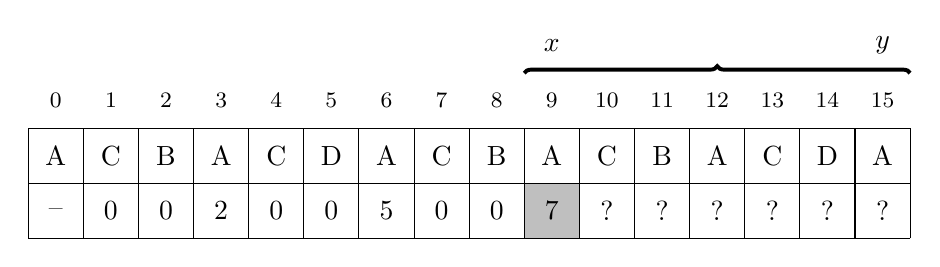
\begin{tikzpicture}[scale=0.7]
\fill[color=lightgray] (9,0) rectangle (10,1);
\draw (0,0) grid (16,2);

\node at (0.5, 1.5) {A};
\node at (1.5, 1.5) {C};
\node at (2.5, 1.5) {B};
\node at (3.5, 1.5) {A};
\node at (4.5, 1.5) {C};
\node at (5.5, 1.5) {D};
\node at (6.5, 1.5) {A};
\node at (7.5, 1.5) {C};
\node at (8.5, 1.5) {B};
\node at (9.5, 1.5) {A};
\node at (10.5, 1.5) {C};
\node at (11.5, 1.5) {B};
\node at (12.5, 1.5) {A};
\node at (13.5, 1.5) {C};
\node at (14.5, 1.5) {D};
\node at (15.5, 1.5) {A};

\node at (0.5, 0.5) {--};
\node at (1.5, 0.5) {0};
\node at (2.5, 0.5) {0};
\node at (3.5, 0.5) {2};
\node at (4.5, 0.5) {0};
\node at (5.5, 0.5) {0};
\node at (6.5, 0.5) {5};
\node at (7.5, 0.5) {0};
\node at (8.5, 0.5) {0};
\node at (9.5, 0.5) {7};
\node at (10.5, 0.5) {?};
\node at (11.5, 0.5) {?};
\node at (12.5, 0.5) {?};
\node at (13.5, 0.5) {?};
\node at (14.5, 0.5) {?};
\node at (15.5, 0.5) {?};

\draw [decoration={brace}, decorate, line width=0.5mm] (9,3.00) -- (16,3.00);

\node at (9.5,3.50) {$x$};
\node at (15.5,3.50) {$y$};


\footnotesize
\node at (0.5, 2.5) {0};
\node at (1.5, 2.5) {1};
\node at (2.5, 2.5) {2};
\node at (3.5, 2.5) {3};
\node at (4.5, 2.5) {4};
\node at (5.5, 2.5) {5};
\node at (6.5, 2.5) {6};
\node at (7.5, 2.5) {7};
\node at (8.5, 2.5) {8};
\node at (9.5, 2.5) {9};
\node at (10.5, 2.5) {10};
\node at (11.5, 2.5) {11};
\node at (12.5, 2.5) {12};
\node at (13.5, 2.5) {13};
\node at (14.5, 2.5) {14};
\node at (15.5, 2.5) {15};

% \draw[thick,<->] (9.5,-0.25) .. controls (9,-1.25) and (4,-1.25) .. (3.5,-0.25);
\end{tikzpicture}
\end{center}

Después de esto, todos los valores restantes de la matriz Z
se pueden determinar utilizando la información
ya almacenada en la matriz Z:

\begin{center}
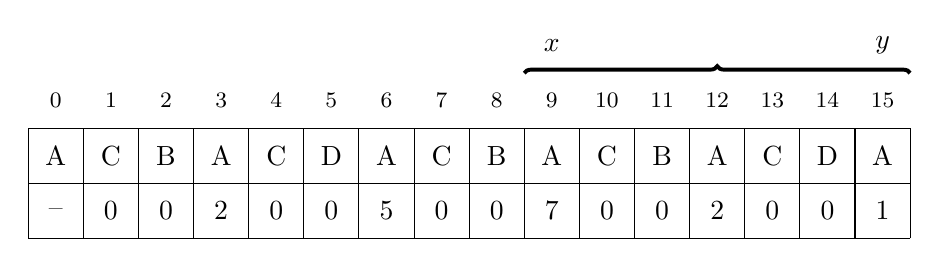
\begin{tikzpicture}[scale=0.7]
\draw (0,0) grid (16,2);

\node at (0.5, 1.5) {A};
\node at (1.5, 1.5) {C};
\node at (2.5, 1.5) {B};
\node at (3.5, 1.5) {A};
\node at (4.5, 1.5) {C};
\node at (5.5, 1.5) {D};
\node at (6.5, 1.5) {A};
\node at (7.5, 1.5) {C};
\node at (8.5, 1.5) {B};
\node at (9.5, 1.5) {A};
\node at (10.5, 1.5) {C};
\node at (11.5, 1.5) {B};
\node at (12.5, 1.5) {A};
\node at (13.5, 1.5) {C};
\node at (14.5, 1.5) {D};
\node at (15.5, 1.5) {A};
\node at (0.5, 0.5) {--};
\node at (1.5, 0.5) {0};
\node at (2.5, 0.5) {0};
\node at (3.5, 0.5) {2};
\node at (4.5, 0.5) {0};
\node at (5.5, 0.5) {0};
\node at (6.5, 0.5) {5};
\node at (7.5, 0.5) {0};
\node at (8.5, 0.5) {0};
\node at (9.5, 0.5) {7};
\node at (10.5, 0.5) {0};
\node at (11.5, 0.5) {0};
\node at (12.5, 0.5) {2};
\node at (13.5, 0.5) {0};
\node at (14.5, 0.5) {0};
\node at (15.5, 0.5) {1};

\draw [decoration={brace}, decorate, line width=0.5mm] (9,3.00) -- (16,3.00);

\node at (9.5,3.50) {$x$};
\node at (15.5,3.50) {$y$};


\footnotesize
\node at (0.5, 2.5) {0};
\node at (1.5, 2.5) {1};
\node at (2.5, 2.5) {2};
\node at (3.5, 2.5) {3};
\node at (4.5, 2.5) {4};
\node at (5.5, 2.5) {5};
\node at (6.5, 2.5) {6};
\node at (7.5, 2.5) {7};
\node at (8.5, 2.5) {8};
\node at (9.5, 2.5) {9};
\node at (10.5, 2.5) {10};
\node at (11.5, 2.5) {11};
\node at (12.5, 2.5) {12};
\node at (13.5, 2.5) {13};
\node at (14.5, 2.5) {14};
\node at (15.5, 2.5) {15};

\end{tikzpicture}
\end{center}

\subsubsection{Usando el arreglo Z}

A menudo es cuestión de gusto si usar
hashing de cadenas o el algoritmo Z.
A diferencia del hashing, el algoritmo Z siempre funciona
y no hay riesgo de colisiones.
Por otro lado, el algoritmo Z es más difícil
de implementar y algunos problemas solo se pueden resolver
usando hashing.

Como ejemplo, considere de nuevo
el problema de coincidencia de patrones,
donde nuestra tarea es encontrar las ocurrencias
de un patrón $p$ en una cadena $s$.
Ya resolvimos este problema de manera eficiente
usando hashing de cadenas, pero el algoritmo Z
proporciona otra forma de resolver el problema.

Una idea habitual en el procesamiento de cadenas es
construir una cadena que consista en
varias cadenas separadas por caracteres especiales.
En este problema, podemos construir una cadena
$p$\texttt{\#}$s$,
donde $p$ y $s$ están separados por un carácter especial
\texttt{\#} que no ocurre
en las cadenas.
El arreglo Z de $p$\texttt{\#}$s$ nos dice las posiciones
donde $p$ ocurre en $s$,
porque esas posiciones contienen la longitud de $p$.

Por ejemplo, si $s=$\texttt{HATTIVATTI} y $p=$\texttt{ATT},
el arreglo Z es el siguiente:

\begin{center}
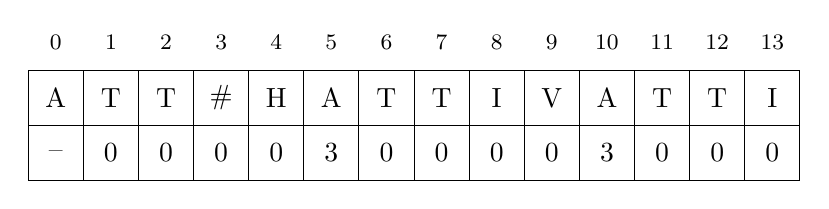
\begin{tikzpicture}[scale=0.7]
\draw (0,0) grid (14,2);

\node at (0.5, 1.5) {A};
\node at (1.5, 1.5) {T};
\node at (2.5, 1.5) {T};
\node at (3.5, 1.5) {\#};
\node at (4.5, 1.5) {H};
\node at (5.5, 1.5) {A};
\node at (6.5, 1.5) {T};
\node at (7.5, 1.5) {T};
\node at (8.5, 1.5) {I};
\node at (9.5, 1.5) {V};
\node at (10.5, 1.5) {A};
\node at (11.5, 1.5) {T};
\node at (12.5, 1.5) {T};
\node at (13.5, 1.5) {I};

\node at (0.5, 0.5) {--};
\node at (1.5, 0.5) {0};
\node at (2.5, 0.5) {0};
\node at (3.5, 0.5) {0};
\node at (4.5, 0.5) {0};
\node at (5.5, 0.5) {3};
\node at (6.5, 0.5) {0};
\node at (7.5, 0.5) {0};
\node at (8.5, 0.5) {0};
\node at (9.5, 0.5) {0};
\node at (10.5, 0.5) {3};
\node at (11.5, 0.5) {0};
\node at (12.5, 0.5) {0};
\node at (13.5, 0.5) {0};

\footnotesize
\node at (0.5, 2.5) {0};
\node at (1.5, 2.5) {1};
\node at (2.5, 2.5) {2};
\node at (3.5, 2.5) {3};
\node at (4.5, 2.5) {4};
\node at (5.5, 2.5) {5};
\node at (6.5, 2.5) {6};
\node at (7.5, 2.5) {7};
\node at (8.5, 2.5) {8};
\node at (9.5, 2.5) {9};
\node at (10.5, 2.5) {10};
\node at (11.5, 2.5) {11};
\node at (12.5, 2.5) {12};
\node at (13.5, 2.5) {13};
\end{tikzpicture}
\end{center}

Las posiciones 5 y 10 contienen el valor 3,
lo que significa que el patrón \texttt{ATT}
ocurre en las posiciones correspondientes
de \texttt{HATTIVATTI}.

La complejidad temporal del algoritmo resultante
es lineal, porque basta con construir
el arreglo Z y recorrer sus valores.

\subsubsection{Implementación}

Aquí hay una breve implementación del algoritmo Z
que devuelve un vector que corresponde al arreglo Z.

\begin{lstlisting}
vector<int> z(string s) {
    int n = s.size();
    vector<int> z(n);
    int x = 0, y = 0;
    for (int i = 1; i < n; i++) {
        z[i] = max(0,min(z[i-x],y-i+1));
        while (i+z[i] < n && s[z[i]] == s[i+z[i]]) {
            x = i; y = i+z[i]; z[i]++;
        }
    }
    return z;
}
\end{lstlisting}

